\documentclass[10pt,a4paper]{article}

\usepackage[T1]{fontenc}
\usepackage[utf8]{inputenc}
\usepackage{charter}
\usepackage[scaled=0.86]{helvet}
\usepackage[a4paper,margin=16mm,top=14mm,bottom=16mm]{geometry}
\usepackage{microtype}
\usepackage{amsmath}
\usepackage{xcolor}
\usepackage{enumitem}
\usepackage{booktabs,tabularx}
\usepackage{titlesec}
\usepackage{caption}
\usepackage{tikz}
\usetikzlibrary{positioning,arrows.meta,fit,backgrounds}
\usepackage[hidelinks]{hyperref}

\definecolor{ink}{HTML}{123A5A}
\definecolor{soft}{HTML}{EEF3F7}

\titleformat{\section}{\sffamily\bfseries\large\color{ink}}{\thesection}{0.6em}{}
\titlespacing*{\section}{0pt}{7pt}{3pt}
\titleformat{\subsection}{\sffamily\bfseries\color{ink}}{\thesubsection}{0.5em}{}
\titlespacing*{\subsection}{0pt}{4pt}{1.5pt}
\setlength{\parindent}{0pt}
\setlength{\parskip}{3pt}
\setlist{nosep,leftmargin=12pt,topsep=1pt}
\captionsetup{font={small,sf},labelfont=bf,skip=3pt}
\renewcommand{\arraystretch}{1.1}
\newcolumntype{L}[1]{>{\raggedright\arraybackslash}p{#1}}
\newcolumntype{Y}{>{\raggedright\arraybackslash}X}

\newcommand{\code}[1]{\texttt{\small #1}}

\begin{document}

{\sffamily
{\LARGE\bfseries\color{ink} IITM Explainable Slotbook: Design Document\par}
\vspace{3pt}
{\normalsize CS5013 course project \quad\textbullet\quad Nishanth S (EE23B049) and Sparsh Gupta (EE23B117)\par}
}
\vspace{-1pt}
{\footnotesize\color{black!60} Written up in November 2026 from our October design notes, the prompt log (P001--P017) and the commit history. It records the plan we started from, so it is in the future tense, and \S4 shows how that plan changed.\par}
\vspace{2pt}
\rule{\linewidth}{0.5pt}

Every semester our department gives each course a lecture slot on the institute timetable grid, mostly by hand-editing last year's slotbook. Nobody can say afterwards why a course got its slot, or what a clash would cost to fix. We will build a tool that produces the slotbook from the rules and preferences directly, never breaks a hard rule, keeps a documented penalty low, and explains every assignment. Alongside it, a small web portal will collect the inputs. We are deliberately leaving some things out: no language model decides or explains anything, rooms are not allocated, the demo portal has no login, and all data in the repository is synthetic.

\section{Architecture}

The system has two halves that meet only at plain CSV files (Figure~\ref{fig:arch}). The \textbf{engine} is a Java 17 program, run from a command line or a small JavaFX viewer. The \textbf{portal} is a set of web pages with serverless functions on Vercel. Keeping the boundary at files means either half can be used, tested or replaced on its own, and a timetabler can always open the files in a spreadsheet.

\begin{figure}[h]
\centering
\resizebox{\linewidth}{!}{%
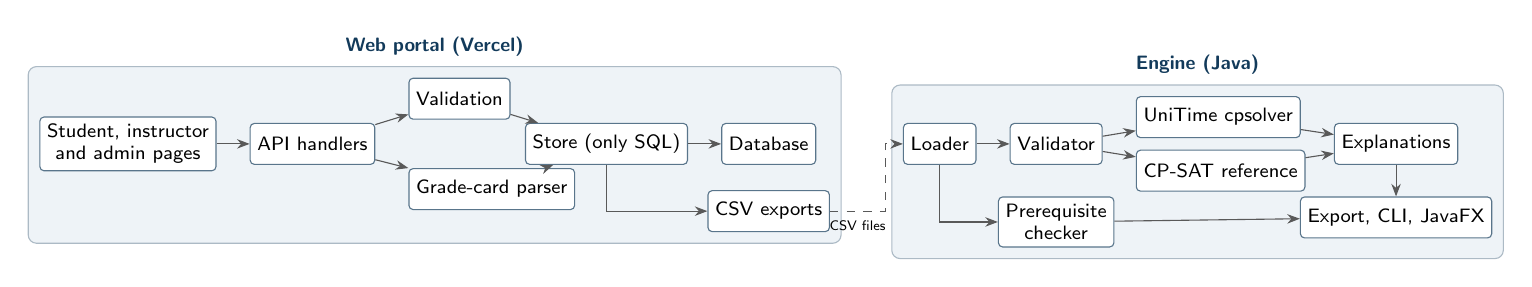
\begin{tikzpicture}[
  font=\sffamily\scriptsize, node distance=3.2mm and 4.2mm,
  box/.style={draw=ink!70, fill=white, rounded corners=1.5pt, inner sep=2.6pt, align=center, minimum height=5.2mm},
  arr/.style={-{Stealth[length=1.6mm]}, draw=black!65},
  grp/.style={draw=ink!35, fill=soft, rounded corners=3pt, inner sep=4pt}]
  \node[box] (forms) {Student, instructor\\and admin pages};
  \node[box, right=of forms] (api) {API handlers};
  \node[box, above right=0.4mm and 4.2mm of api] (val) {Validation};
  \node[box, below right=0.4mm and 4.2mm of api] (gc) {Grade-card parser};
  \node[box, right=19mm of api] (store) {Store (only SQL)};
  \node[box, right=of store] (db) {Database};
  \node[box, below=of db] (exp) {CSV exports};
  \draw[arr] (forms) -- (api); \draw[arr] (api) -- (val); \draw[arr] (api) -- (gc);
  \draw[arr] (val) -- (store); \draw[arr] (gc) -- (store); \draw[arr] (store) -- (db);
  \draw[arr] (store) |- (exp);
  \node[box, right=11mm of db] (load) {Loader};
  \node[box, right=of load] (vj) {Validator};
  \node[box, right=of vj, yshift=3.4mm] (uni) {UniTime cpsolver};
  \node[box, right=of vj, yshift=-3.4mm] (cps) {CP-SAT reference};
  \node[box, right=of uni, yshift=-3.4mm] (ex) {Explanations};
  \node[box, below=4mm of ex] (out) {Export, CLI, JavaFX};
  \node[box, below=4mm of vj] (pc) {Prerequisite\\checker};
  \draw[arr] (load) -- (vj); \draw[arr] (vj) -- (uni); \draw[arr] (vj) -- (cps);
  \draw[arr] (uni) -- (ex); \draw[arr] (cps) -- (ex); \draw[arr] (ex) -- (out);
  \draw[arr] (load) |- (pc); \draw[arr] (pc) -- (out);
  \draw[arr, dashed] (exp.east) -- node[below, font=\sffamily\tiny]{CSV files} ++(7mm,0) |- (load.west);
  \begin{scope}[on background layer]
    \node[grp, fit=(forms)(val)(gc)(db)(exp), label={[font=\sffamily\scriptsize\bfseries, text=ink]above:Web portal (Vercel)}] {};
    \node[grp, fit=(load)(uni)(cps)(out)(pc), label={[font=\sffamily\scriptsize\bfseries, text=ink]above:Engine (Java)}] {};
  \end{scope}
\end{tikzpicture}}
\caption{Architecture. Data flows left to right; the dashed arrow is the only link between the two halves.}
\label{fig:arch}
\end{figure}

\vspace{-5pt}
\textbf{Engine.} Data flows one way: load, validate, solve, explain, export. Validation runs before any solving, and reports every problem with a specific code (e.g.\ \code{FIXED\_CONFLICT}). Invalid input is never solved. Clashes are computed from real meeting times on the official IITM grid, since slots with different letters can overlap. The hard rules are:
\begin{itemize}
\item one slot per course, taken from its allowed set (or its fixed slot);
\item no lecture over the course's own lab;
\item no overlap between protected pairs of courses;
\item no instructor teaching two overlapping meetings;
\item no two lectures in the same room at once.
\end{itemize}

\textbf{One objective, shared.} A single \code{Objective} class defines the penalty, and every solver and the explanation code use it. A course costs the instructor's penalty for its slot (0--100, and 1 if they gave none), plus 2 if it moves away from last year's slot. Each overlapping pair costs 3 per overlapping meeting, times the pair's weight. The weight sums $\max(1,\,4-\text{worse rank})$ over the students taking both courses, so a clash between top choices hurts most.

\textbf{Solvers behind an interface.} We will start with an exact CP-SAT model (OR-Tools), which can prove optimality on small inputs. We then plan to wrap UniTime's \emph{cpsolver} library, a local-search engine proven on real university timetables, and make it the default for scale. CP-SAT stays as the yardstick, so the heuristic's gap from the optimum is measured, not assumed.

\textbf{Explanations from the model, not the solver.} After solving, we recompute everything from the problem and the final assignment. For the chosen slot we give the rules it satisfies and the penalties it pays. For every other slot we give the rule it breaks, or its estimated extra cost. Because the explanation code never looks inside the solver, explanations are identical whichever solver ran.

\textbf{Portal.} Requests pass through pure validation code into a store module, the only code that touches the database; every query is parameterised. Storage starts as a Google Sheet for the demo, and moves to Postgres once we need relational rules and concurrent writers. There, the validation rules are repeated as foreign keys and \code{CHECK} constraints, and each replacing write is one transaction. Prerequisites are advisory: a student's uploaded grade card is parsed (grades U, W and I don't count as completed), missing prerequisites produce warnings, and nothing is blocked or sent to the solver.

\section{Module split}

Each module has one job, and dependencies point one way: \code{model} depends on nothing, and everything else depends on \code{model}. The CLI and the viewer share \code{service}, so neither contains solver logic.

\begin{tabularx}{\linewidth}{@{}L{25mm}L{52mm}Y@{}}
\toprule
\textbf{Module} & \textbf{Main classes} & \textbf{Responsibility}\\
\midrule
\multicolumn{3}{@{}l}{\sffamily\bfseries\small\color{ink} Engine (\code{in.ac.iitm.slotbook})}\\
\code{model} & \code{Course}, \code{Slot}, \code{TimeGrid}, \code{TimetableProblem}, \code{TimetableSolution} & Immutable records; real meeting times; student pair weights\\
\code{io} & \code{DatasetLoader}, \code{CsvSupport}, \code{SlotbookExporter}, \code{PrerequisiteLoader} & Read the five CSVs (plus optional prerequisite files) and write the exports\\
\code{validation} & \code{InputValidator}, \code{PrerequisiteChecker} & Reject invalid input with coded issues; compute advisory prerequisite warnings\\
\code{solver} & \code{TimetableSolver}, \code{Objective}, \code{OrToolsTimetableSolver}, \code{unitime/*} & The solver interface, the shared objective, CP-SAT, and the cpsolver mapping and search\\
\code{explain} & \code{ExplanationBuilder} & Per-course reasons and classified alternatives\\
\code{service}, \code{cli}, \code{ui} & \code{SlotbookService}, \code{SlotbookCli}, \code{SlotbookApplication} & One facade; command line and JavaFX on top of it\\
\code{testing} (tests) & \code{ConstraintChecker}, \code{PenaltyCalculator}, \code{BruteForceSolver}, \code{ScenarioGenerator} & Independent oracles and generated scenarios, kept out of production code\\
\midrule
\multicolumn{3}{@{}l}{\sffamily\bfseries\small\color{ink} Portal (\code{portal/})}\\
\code{api/*.js} & \code{submit}, \code{admin}, \code{results}, \code{solver}, \code{health} & HTTP handlers: parse, call domain and store, map errors to status codes\\
domain & \code{\_validation}, \code{\_gradecard}, \code{\_prerequisites}, \code{\_completions} & Pure rules; the grade-card parser; the completion-source registry\\
storage & \code{\_store}, \code{\_db}, \code{db/migrations} & All SQL; connection pool; numbered schema changes\\
\code{public/} & Student, professor, admin and results pages & Forms and dashboards; no business rules in the browser\\
\bottomrule
\end{tabularx}

\section{Test plan}

We test against oracles written separately from the code under test, rather than asking the code whether it is right.

\begin{tabularx}{\linewidth}{@{}L{25mm}Y L{52mm}@{}}
\toprule
\textbf{Level} & \textbf{What we test} & \textbf{Checked against}\\
\midrule
Unit & CSV parsing, every validation code, the objective, explanations, grade-card rows, the prerequisite rule & Hand-computed expected values\\
Solver correctness & Both solvers on fixed fixtures and randomly generated scenarios & Independent constraint checker and penalty calculator\\
Optimality & CP-SAT on small seeded problems & Exhaustive brute-force search\\
Cross-solver & cpsolver against CP-SAT on every scenario & CP-SAT's proven optimum; gap recorded\\
Contract & Portal CSV exports; portal against CLI prerequisite warnings & Engine's loader headers; one shared golden file\\
Integration & Store on a real Postgres: rollback, concurrency, constraints & Database state afterwards\\
Stress & Seeded random input, corrupted PDFs, large volumes, hundreds of simultaneous requests & Invariants (never a 500 or a half-written submission); naive re-implementations\\
Manual & JavaFX viewer; portal pages in a browser, console errors included & A checklist\\
\bottomrule
\end{tabularx}

\vspace{2pt}
Four rules apply throughout:
\begin{itemize}
\item Never assert one exact timetable when several are equally good.
\item Seed every random test, so a failure can be replayed.
\item Show that every bug-fix test fails on the old code.
\item List every test, with what it checks, in the test plan.
\end{itemize}
GitHub Actions runs the Java suite, the portal suites (with a Postgres service), CLI runs with both solvers, and a man-page check on every push and pull request.

\section{Revised milestone plan}

Our first plan (prompts P001--P005) ran straight to the mid-evaluation: architecture and synthetic data, the CP-SAT engine with explanations, tests, then evaluator documentation. We revised it as we learned. Comparing our model with UniTime showed that its search scales much better, and that our first engine missed a room clash and used approximate slot times, so we added a cpsolver milestone with real IITM meeting times. Typing preferences up by hand was clearly going to be the bottleneck, so we added the portal. Later, concurrent writers and prerequisites made relational storage necessary, so Postgres replaced the Sheet. Finally, we added a hardening milestone before deployment.

\begin{tabularx}{\linewidth}{@{}L{8mm}L{37mm}Y L{24mm}@{}}
\toprule
& \textbf{Milestone} & \textbf{Done when} & \textbf{Change from first plan}\\
\midrule
M1 & Engine v1: CP-SAT, explanations, CLI, JavaFX, CI & Feasible fixture solves; infeasible one reports \code{FIXED\_CONFLICT}; hard rules hold on every output & As planned\\
M2 & Testing framework & CP-SAT equals brute force on every seed; oracles agree with both solvers & Expanded (oracles, generated scenarios)\\
M3 & Engine v2: cpsolver default, real IITM times, rooms, labs & cpsolver's score equals our objective; gap from CP-SAT measured on all scenarios & \textbf{New} (after the UniTime comparison)\\
M4 & Demo portal on Google Sheets & Exports match the engine's CSVs byte for byte & \textbf{New}\\
M5 & Mid-evaluation & Showcase dataset, three-page practices PDF, live code change rehearsed & As planned\\
M6 & v3: Postgres, grade-card prerequisite warnings, man page & Portal and CLI warnings equal the golden file; integration tests pass on Postgres & \textbf{New} (replaces the Sheet)\\
M7 & Hardening and deployment & No server errors under stress; deployed with a configured database & \textbf{New}\\
\bottomrule
\end{tabularx}

\vspace{2pt}
\textbf{Main risks.} The heuristic may fall short of the optimum; CP-SAT stays as the yardstick. Our objective could drift from cpsolver's score, so a test checks they are equal. Simultaneous submissions could corrupt data; transactions, constraints and stress tests guard against that. Real student data must never reach the repository: test grade cards are generated and marked, and a check rejects any that aren't. Until there is institute login and a consent policy, the portal collects no real data.

\end{document}
